\documentclass[a4paper,12pt]{article}

\usepackage{cmap}
\usepackage{mathtext}
\usepackage[T2A]{fontenc}
\usepackage[utf8]{inputenc}
\usepackage[english,russian]{babel}
\usepackage{listings}

\usepackage{amsmath,amsfonts,amssymb,amsthm,mathtools}
\usepackage{icomma}
\usepackage{upgreek}
\mathtoolsset{showonlyrefs=true}

\usepackage{tabto}
\usepackage{euscript}
\usepackage{mathrsfs}

\usepackage[top=3cm, bottom=1.5cm]{geometry}
\usepackage{graphicx}

\newcommand*{\hm}[1]{#1\nobreak\discretionary{}
{\hbox{$\mathsurround=0pt #1$}}{}}

\author{Kupriyanov Kirill}
\title{Data Analysis PI\\Theoretical assignment $\#7$}
\date{}

\begin{document}
\maketitle
\thispagestyle{empty}
\newpage
\section*{Task 1.}
\underline{\textit{Problem:}} Does the principal component analysis (PCA) transformation require the preliminary feature standartization
procedures (centering / scaling)? Explain your answer.\\
\newline
\underline{\textit{Solution:}} Перед использованием метода главных компонент
предпочтительнее предварительно стандартизировать данные. Так как за основу
метода взята дисперсия, масштабирование величин приведет к изменению главных
компонент и как следствие результатов. Если какая-то величина будет измеряться
гораздо большими числами, чем другая, то эта величина будет доминировать и, в
основном, именно она будет влиять на результат. Это можно воспринимать как
весы, и если такого в решаемой задаче не предполагается, то лучше данные
стандартизировать.

\newpage
\section*{Task 4.}
\underline{\textit{Problem:}} Provide an example of the two-dimensional \((d =
2)\) dataset in the binary classification problem for which the preliminary
application of PCA compression to dimensionality \(d = 1\) would hurt the
classification accuracy dramatically. Explain, why PCA can hurt the
classification accuracy?\\
\newline
\underline{\textit{Solution:}} Допустим у нас следующее распределение. Красным выделены объекты одного класса, зеленым
другого.
\begin{center}
    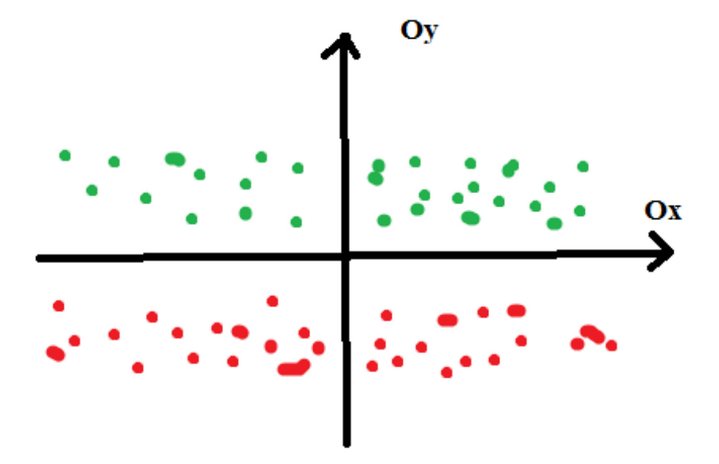
\includegraphics[width=0.8\linewidth]{1.png}
\end{center}
В таком случае главная компонента будет примерно совпадать с осью Ox. Если мы
спроектируем объекты на такую главную компоненту, то получим следующую картину:
\begin{center}
    
\includegraphics[width=0.8\linewidth]{2.png}
\end{center}
В итоге, получилась смесь точек, которую невозможно адекватно классифицировать.
Получается это в следствие того, что выборка вытянута по оси Ox, как следствие
выбирается главная компонента схожая с Ox. Но ключевая информация о разделении
классов находится на
оси Oy. Иначе говоря, в этом примере, проектируя объекты, мы теряем всю
информацию о классификации.

\end{document}


% EOF

